\documentclass[12pt,border=4pt,multi]{article}%\documentclass[tikz,border=4pt,multi]{article}
\usepackage{lingmacros}
\usepackage{tree-dvips}
\usepackage{amssymb} %for mathbb{}
\usepackage[dvipsnames]{xcolor}
\usepackage{forest}
\usepackage{amsmath} %for matrices
\usepackage{xeCJK}
\usepackage{tikz}
\usepackage[arrowdel]{physics}
\usepackage{graphicx}
\usepackage{wrapfig}
\usepackage{listings}
\usepackage{pgfplots, pgfplotstable}
\graphicspath{{./img}} %specify the graphics path to be relative to the main .tex file, denoting the main .tex file directory as ./
\newcommand\Myperm[2][^n]{\prescript{#1\mkern-2.5mu}{}P_{#2}}
\newcommand\Mycomb[2][^n]{\prescript{#1\mkern-0.5mu}{}C_{#2}}
\definecolor{orchid}{rgb}{0.7, 0.4, 1.1}

\begin{document}

\section*{Xi Liu, xl3504, Homework 5}
Problem 1\\
since $X \in \{0,\; 1,\; ...,\; N\} = \{a_0,\; a_1,\; ...,\; a_N\}$\\
expectation of a discrete random variable $X$ with the values $a_1, a_2$, ...
\begin{align*}
E(X) &= \sum_i a_i P(X = a_i)\\
&= \sum_{n = 0}^N a_n\, P(X = a_n)\\
&= \sum_{n = 0}^N n\, P(X = n)\\
\end{align*}
\begin{figure}[h!]
	\centering
	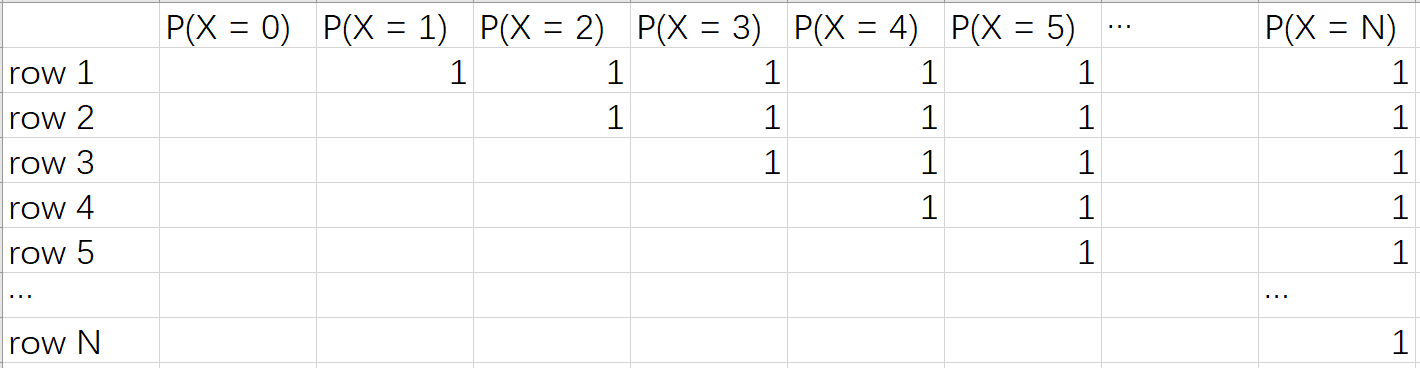
\includegraphics[width=1.1\textwidth, height=0.55\textwidth]{1} %img size
\end{figure}\\
for each column of $P(X = n)$, its contribution to the expected value is $n P(X = n)$, in which $n$ is equal to the sum of 1's in each column of $P(X = n)$\\
\[\sum_{n = 0}^N n\, P(X = n) = \sum_{i = 1}^N \text{(contribution from row $i$)}\]
\\
using summation by parts
\begin{align*}
E(X) &= \sum_{n = 0}^N n\, P(X = n)\\
&= \sum_{n = 1}^N P(X = n) + \sum_{n = 2}^N P(X = n)\\
&\qquad + \sum_{n = 3}^N P(X = n) + ... + \sum_{n = N}^N P(X = n)\\
&= \sum_{n = 0}^{N - 1}\left(\sum_{i = n}^N P(X = i)\right)\\
&= \sum_{n = 0}^{N - 1} P(X > n)\\
&\text{/* since } P(X > n) = \sum_{i = n}^N P(X = i) \text{ */}\\
\end{align*}
\\
\\
\\
\\
\newpage 
\noindent
Problem 2\\
1. 
\begin{align*}
a := x\\
F(a) &= P(X \leq a)\\
&= \int_{-\infty}^{a} f(x) dx\\
&= \int_{0}^{a} \left(2Kxe^{-Kx^2}\right) dx\\ 
\text{/* } &u := -Kx^2\\
&du = -2Kxdx\\
&-du = 2Kxdx\\ 
&-\int e^u du = -e^u \text{ */}\\
&= \left[-e^{-Kx^2}\right]_0^a\\
&= -\left[e^{-Kx^2}\right]_0^a\\
&= -\left(e^{-Ka^2} - e^0\right)\\
&= -\left(e^{-Ka^2} - 1\right)\\
&= 1 - e^{-Ka^2}\\
&=  1 - e^{-Kx^2}\\
\end{align*}
\begin{center}
$ \boxed{F(x) =
\begin{cases}
1 - e^{-Kx^2} & \text{if } x > 0\\
0 & \text{otherwise}\\
\end{cases}}$
\end{center}
\\
\\
\\
\\
\newpage
\noindent
2.\\
mean = $E[X]$
\begin{align*}
E[X] &= \int_{-\infty}^{\infty} x f(x) dx\\
&=  \int_{0}^{\infty} x \left(2Kxe^{-Kx^2}\right) dx\\
&=  \int_{0}^{\infty} \left(2Kx^2e^{-Kx^2}\right) dx\\
&=  2K\int_{0}^{\infty} x^2e^{-Kx^2} dx\\
&\text{/* see calculations in next page */}\\
&= 2K(I_1)\\
&= 2K\left(\frac{1}{2K}I_2\right)\\
&= I_2\\
&= \boxed{\sqrt{\frac{\pi}{4K}}}\\
\end{align*}
\begin{figure}
	\centering
	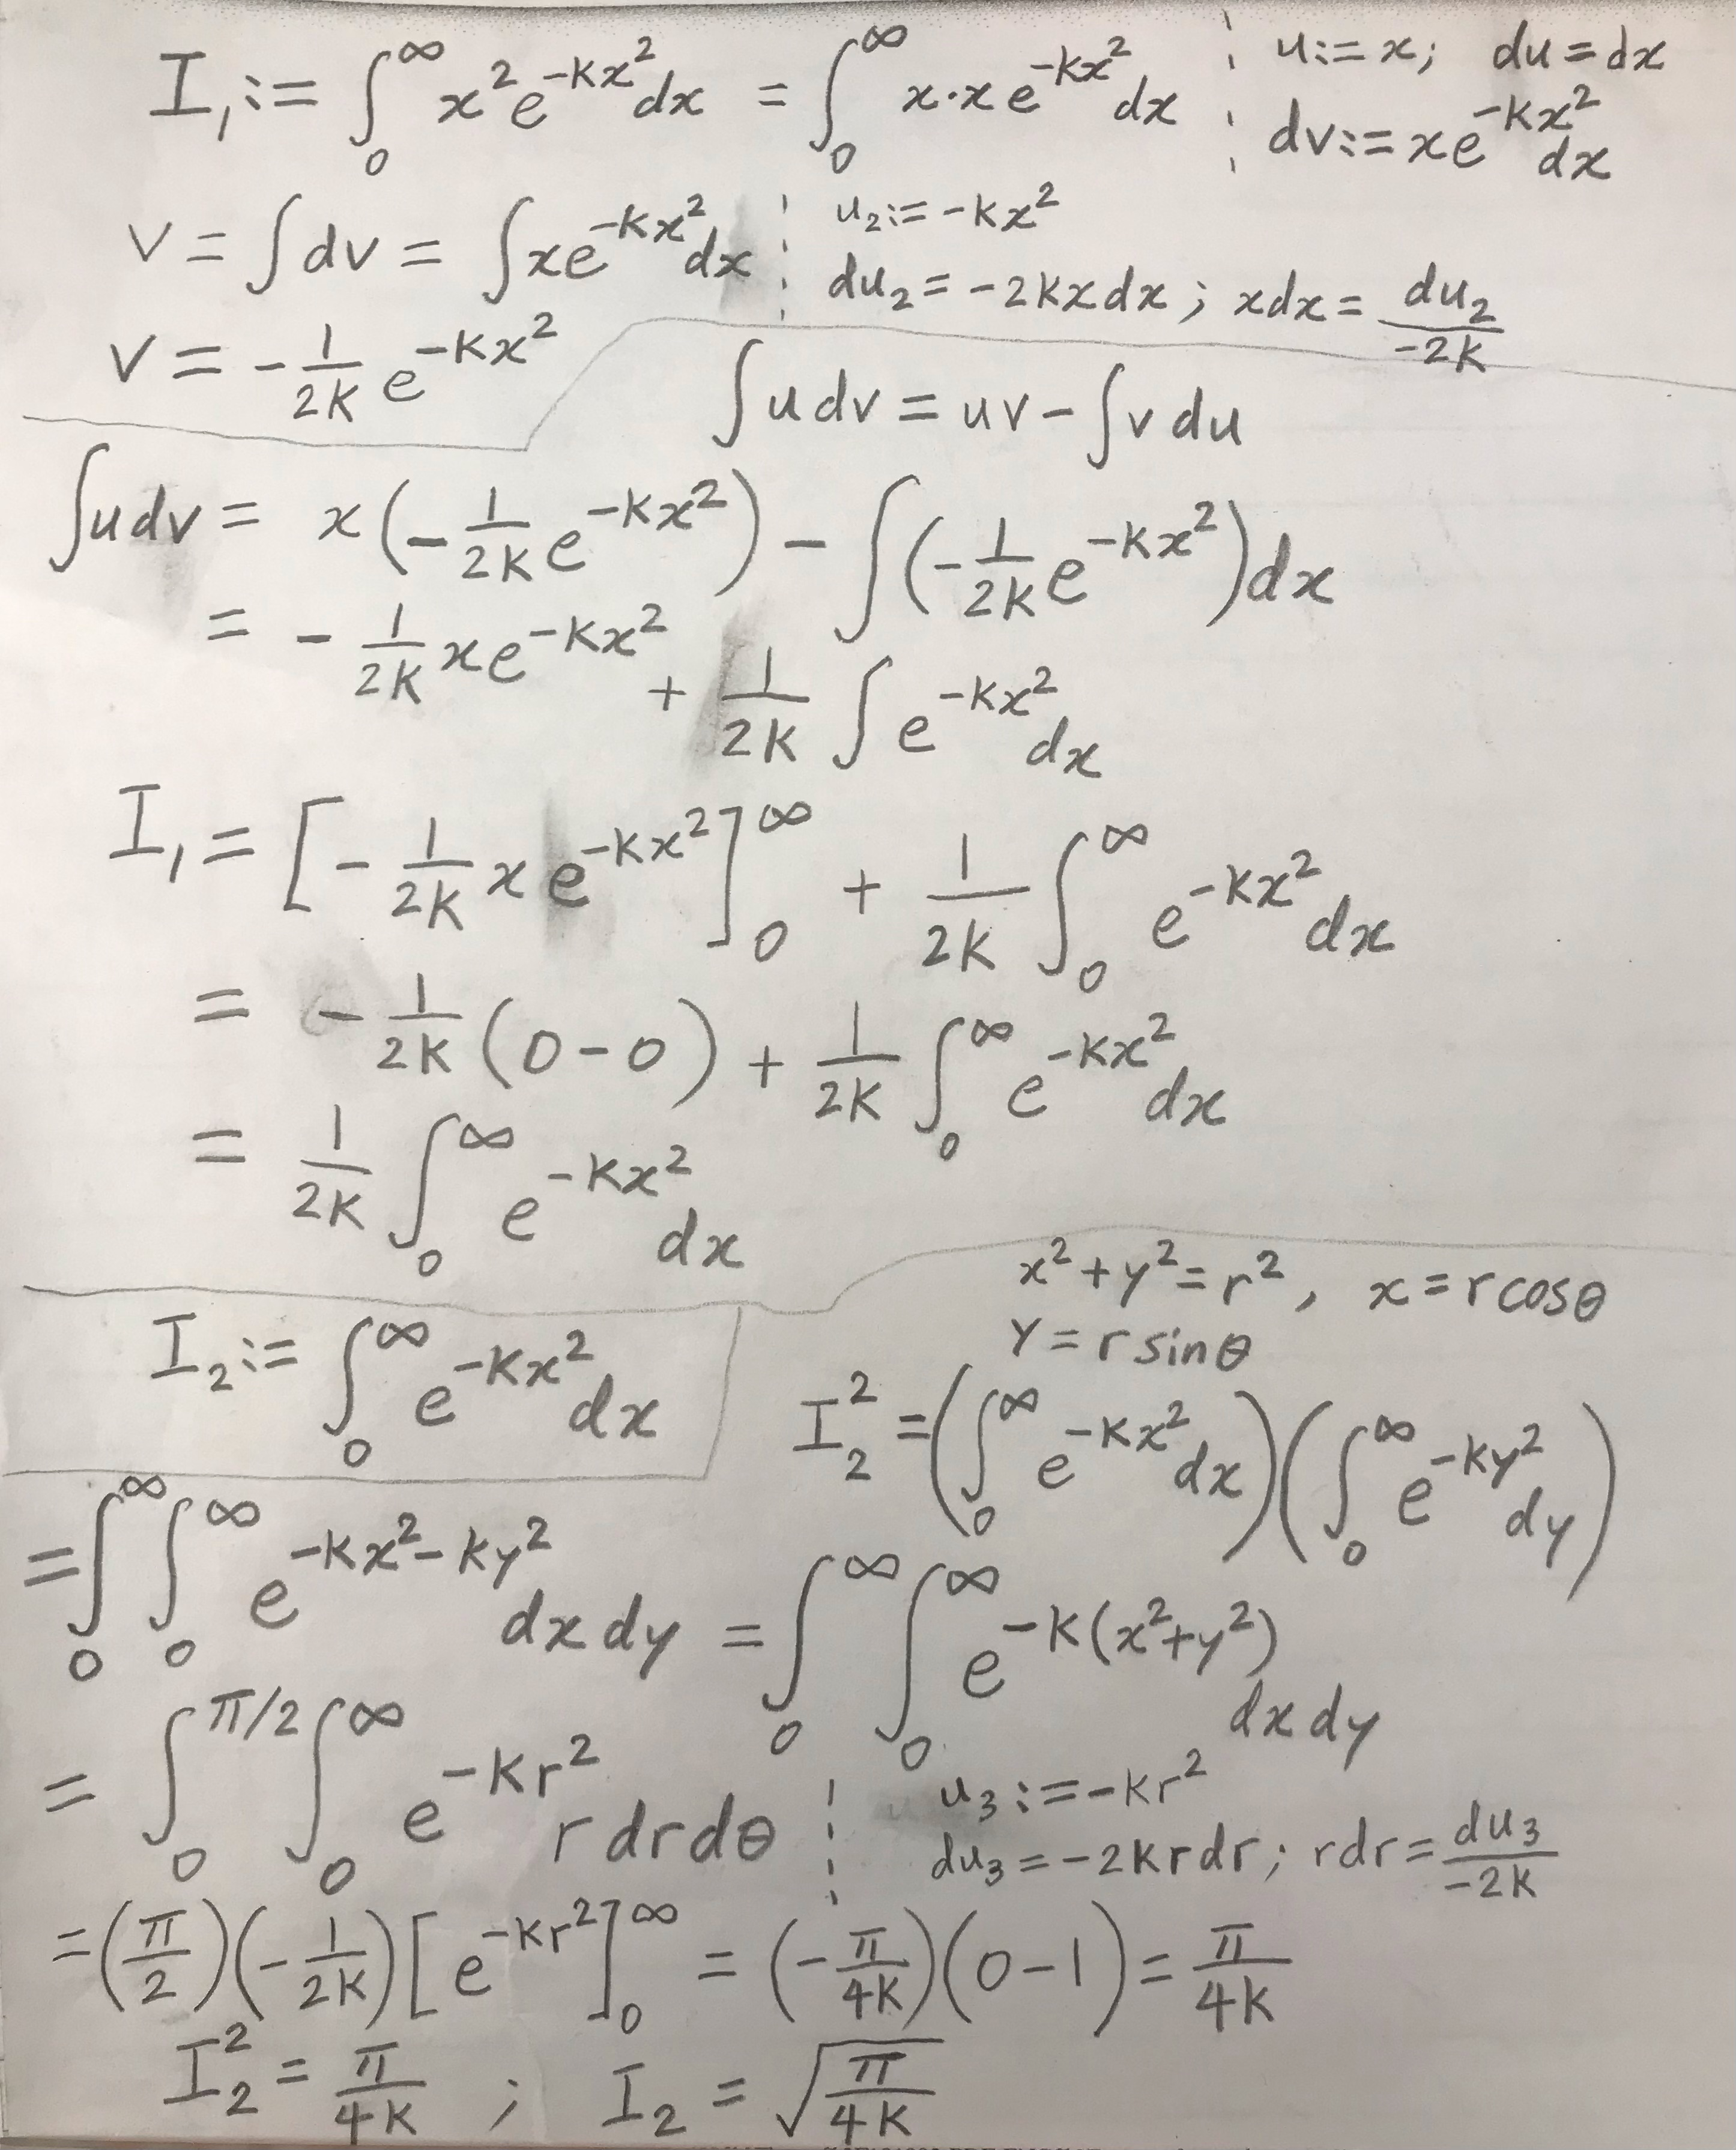
\includegraphics[width=1.1\textwidth, height=1.4\textwidth]{2.2} %img size
\end{figure}\\
\\
\\
\\
\\
\\
\\
\\
\\
\\
\\
\\
\\
\\
\\
\\
alternatively, the calculation of $I_2$ can be done as follows:\\
a continuous random variable has a normal distribution with parameters $\mu$ and $\sigma^2 > 0$ if its probability density function is given by
{\large
\begin{align*}
f(x) &= \frac{1}{\sqrt{2\pi\sigma^2}} e^{-\frac{1}{2}\left(\frac{x - \mu}{\sigma}\right)^2}\\
\end{align*}}
\begin{align*}
\int_{-\infty}^{\infty} f(x) dx &= \int_{-\infty}^{\infty} \frac{1}{\sqrt{2\pi\sigma^2}} e^{-\frac{1}{2}\left(\frac{x - \mu}{\sigma}\right)^2} dx\\
&= \frac{1}{\sqrt{2\pi\sigma^2}} \int_{-\infty}^{\infty} e^{-\frac{1}{2}\left(\frac{x - \mu}{\sigma}\right)^2} dx\\
\text{/* set } \mu = 0; \qquad K &= \frac{1}{2\sigma^2}; \qquad \sigma = \frac{1}{\sqrt{2K}} \text{*/}\\
&= \frac{1}{\sqrt{2\pi(1/\sqrt{2K})^2}} \int_{-\infty}^{\infty} e^{-\frac{1}{2}\left(\frac{x - 0}{1/(\sqrt{2K})}\right)^2} dx\\
&= \frac{1}{\sqrt{2\pi}(1/\sqrt{2K})} \int_{-\infty}^{\infty} e^{-\frac{1}{2}\left(\sqrt{2K}x\right)^2} dx\\
&= \frac{\sqrt{2K}}{\sqrt{2\pi}} \int_{-\infty}^{\infty} e^{-\frac{1}{2}\left(2Kx^2\right)} dx\\
&= \sqrt{\frac{K}{\pi}} \int_{-\infty}^{\infty} e^{-Kx^2} dx = 1\\
\text{/* since } \int_{-\infty}^{\infty} f(x)dx  = 1 &\text{ for a $f$ that is the probability density}\\
&\text{function of a continuous random variable $X$}\text{ */}\\
\int_{-\infty}^{\infty} e^{-Kx^2} dx &= \sqrt{\frac{\pi}{K}}\\
\end{align*}
\begin{align*}
\text{/* since } f(x) = e^{-Kx^2} &\text{is an even function */}\\
\int_{-\infty}^{\infty} e^{-Kx^2} dx &= 2\int_0^{\infty} e^{-Kx^2} dx\\
\sqrt{\frac{\pi}{K}} &=  2\int_0^{\infty} e^{-Kx^2} dx\\
\int_0^{\infty} e^{-Kx^2} dx &= \frac{1}{2}\sqrt{\frac{\pi}{K}}\\
&= \sqrt{\frac{1}{4}}\sqrt{\frac{\pi}{K}}\\
&= \sqrt{\frac{\pi}{4K}} = I_2\\
\end{align*}
variance = $Var(X)$
\begin{align*}
Var(X) &= E[X^2] - E[X]^2\\
\end{align*}
\begin{align*}
E[g(X)] &= \int_{-\infty}^{\infty} g(x) f_X(x) dx\\ 
E[X^2] &= \int_{-\infty}^{\infty} x^2 f(x) dx\\
&=  \int_{0}^{\infty} x^2 \left(2Kxe^{-Kx^2}\right) dx\\
&= 2K\int_{0}^{\infty} x^3 e^{-Kx^2} dx\\
&\text{/* see calculations in next page */}\\
&= 2K(I_3)\\
&= 2K\left(\frac{1}{2K^2}\right)\\
&= \frac{1}{K}\\
\end{align*}
\\
\\
\\
\begin{align*}
I_3 &:= \int_0^{\infty} x^3 e^{-Kx^2} dx\\
&= \int_0^{\infty} x^2 \cdot x e^{-Kx^2} dx\\
u &:= x^2; \qquad du = 2xdx; \qquad dv := xe^{-Kx^2}dx\\
v &= \int dv = \int xe^{-kx^2} dx\\
u_2 &:= -Kx^2; \qquad du_2 = -2Kxdx; \qquad xdx = -\frac{1}{2K}du_2\\
v &= -\frac{1}{2K}\int e^{u_2} du_2 = -\frac{1}{2K}e^{-Kx^2}\\
\int udv &= uv - \int vdu\\
&= x^2\left(-\frac{1}{2K}e^{-Kx^2}\right) - \int\left(-\frac{1}{2K}e^{-Kx^2}\right)\left(2xdx\right)\\
&= -\frac{1}{2K}x^2e^{-Kx^2} + \int\frac{1}{K}xe^{-Kx^2}dx\\
I_3 &= \left[-\frac{1}{2K}x^2e^{-Kx^2}\right]_0^{\infty} + \int_0^{\infty}\frac{1}{K}xe^{-Kx^2}dx\\
\end{align*}
\begin{align*}
&\text{/* since } \forall a \in \mathbb{R},\;\lim_{x \rightarrow \infty} \frac{e^x}{x^a} > 0\\
&\text{the exponential function $e^x$ is an asymptotic upper bound}\\
&\text{on the polynomial function $x^a$ */}\\
I_3 &= -\frac{1}{2K}(0 - 0) + \int_0^{\infty}\frac{1}{K}xe^{-Kx^2}dx\\
&= \int_0^{\infty}\frac{1}{K}xe^{-Kx^2}dx\\
&= \frac{1}{K}\int_0^{\infty}xe^{-Kx^2}dx\\
\text{/* } u &:= -Kx^2; \qquad du = -2Kxdx; \qquad xdx = \frac{du}{-2K}\\
\frac{1}{K}\int xe^{-Kx^2}dx &= \frac{1}{K}\cdot\frac{1}{-2K}e^{-Kx^2}
= \frac{1}{-2K^2}e^{-Kx^2}\\
\text{ */}\\
I_3 &= \left[-\frac{1}{2K^2}e^{-Kx^2}\right]_0^{\infty}\\
&= -\frac{1}{2K^2}(0 - 1)\\
&= \frac{1}{2K^2}\\
\end{align*}
\\
\\
\begin{align*}
Var(X) &= E[X^2] - E[X]^2\\
&= \frac{1}{K} - \left(\sqrt{\frac{\pi}{4K}}\right)^2\\
&= \frac{1}{K} - \frac{\pi}{4K}\\
&= \boxed{\frac{4 - \pi}{4K}}\\
\end{align*}
\\
\\
\\
\\
\\
3.\\
let $F_Y(a)$ be the cumulative distribution function of $Y$
\begin{align*}
F_Y(y) &= P(Y \leq y)\\
&= P(KX^2 \leq y)\\
&= P(X \leq \sqrt{\frac{y}{K}})\\
&= 1 - e^{-K\left(\sqrt{y/K}\right)^2}\\
&= 1 - e^{-K(y/K)}\\
&= \boxed{1 - e^{-y}}\\
\end{align*}
let $f_Y(x)$ be the probability density function of $Y$\\
\begin{align*}
f_Y(x) &= \frac{d}{dy}\left(F_Y(y)\right)\\
&= \frac{d}{dy}\left(1 - e^{-y}\right)\\
&= (-1)(-e^{-y})\\
&= e^{-y}\\
\end{align*}
\begin{center}
$\boxed{
f_Y(x) =
\begin{cases}
e^{-y} & \text{if } y > 0\\
0 & \text{otherwise}\\
\end{cases}
}$
\end{center}
\newpage
\noindent
Problem 3\\
1.\\
mean = $E[X]$
\begin{align*}
E[X] &= \int_{-\infty}^{\infty} xf(x) dx\\
&= \int_0^{\infty} x\left(\lambda e^{-\lambda x}\right) dx\\
&= \lambda\int_0^{\infty} xe^{-\lambda x} dx\\
&\text{/* see calculations in next page */}\\
&= \lambda(I_6)\\
&= \lambda\left(\frac{1}{\lambda^2}\right)\\
&= \boxed{\frac{1}{\lambda}}\\
\end{align*}
\begin{align*}
I_6 &:= \int_0^{\infty} xe^{-\lambda x} dx\\
&u := x;\qquad du = dx;\qquad dv := e^{-\lambda x}dx\\
v &= \int dv = \int e^{-\lambda x}dx\\
&u_2 := -\lambda x; \qquad du_2 = -\lambda dx; \qquad dx = \frac{du_2}{-\lambda}\\
v &= -\frac{1}{\lambda} e^{-\lambda x}\\
\int udv &= uv - \int vdu\\
&= x\left( -\frac{1}{\lambda} e^{-\lambda x}\right) + \int\left( -\frac{1}{\lambda} e^{-\lambda x}\right)dx\\
&= -\frac{1}{\lambda} xe^{-\lambda x} - \frac{1}{\lambda}\int e^{-\lambda x}dx\\
u &= -\lambda x; \qquad du = -\lambda dx; \qquad dx = \frac{du}{-\lambda}\\ 
I_6 &= \left[-\frac{1}{\lambda} xe^{-\lambda x}\right]_0^{\infty} + \left(\frac{1}{\lambda^2}\right)\left[e^{-\lambda x}\right]_0^{\infty}\\
&= \left(-\frac{1}{\lambda}\right)\left(0 - 0\right) + \left(\frac{1}{\lambda^2}\right)\left(0 - 1\right)\\
&= \frac{1}{\lambda^2}\\
\end{align*}
\newpage
\noindent
2.\\
variance = $Var(X)$\\
\begin{align*}
Var(X) &= E[X^2] - E[X]^2\\
\end{align*}
\begin{align*}
E[g(X)] &= \int_{-\infty}^{\infty} g(x) f_X(x) dx\\ 
E[X^2] &= \int_{-\infty}^{\infty} x^2 f(x) dx\\
&= \int_0^{\infty} x^2\left(\lambda e^{-\lambda x}\right)dx\\
&= \lambda \int_0^{\infty} x^2 e^{-\lambda x}dx\\
&\text{/* see calculations in next page */}\\
&= \lambda (I_7)\\
&= \lambda \left(\frac{2}{\lambda^3}\right)\\
&= \frac{2}{\lambda^2}\\
\end{align*}
\begin{align*}
Var(X) &= E[X^2] - E[X]^2\\
&= \frac{2}{\lambda^2} - \left(\frac{1}{\lambda}\right)^2\\
&= \frac{2}{\lambda^2} - \frac{1}{\lambda^2}\\
&= \boxed{\frac{1}{\lambda^2}}\\
\end{align*}
\begin{align*}
I_7 &:= \int_0^{\infty} x^2e^{-\lambda x} dx\\
&u := x^2;\qquad du = 2xdx;\qquad dv := e^{-\lambda x}dx\\
v &= \int dv = \int e^{-\lambda x}dx\\
&u_2 := -\lambda x; \qquad du_2 = -\lambda dx; \qquad dx = \frac{du_2}{-\lambda}\\
v &= -\frac{1}{\lambda} e^{-\lambda x}\\
\end{align*}
\begin{align*}
\int udv &= uv - \int vdu\\
&= x^2\left( -\frac{1}{\lambda} e^{-\lambda x}\right) + \int\left( -\frac{1}{\lambda} e^{-\lambda x}\right)\left(2xdx\right)\\
&= -\frac{1}{\lambda} x^2e^{-\lambda x} - \frac{2}{\lambda}\int xe^{-\lambda x}dx\\
&\text{\qquad/* from previous calculation of $I_6$, we know }\\
&\text{\qquad}\int xe^{-\lambda x}dx= -\frac{1}{\lambda} xe^{-\lambda x} + \frac{1}{\lambda^2}e^{-\lambda x} \text{ */}\\ 
&= -\frac{1}{\lambda} x^2e^{-\lambda x} - \frac{2}{\lambda}\left(-\frac{1}{\lambda} xe^{-\lambda x} + \frac{1}{\lambda^2}e^{-\lambda x}\right)\\
&= -\frac{1}{\lambda} x^2e^{-\lambda x} + \frac{2}{\lambda^2}xe^{-\lambda x} - \frac{2}{\lambda^3}e^{-\lambda x}\\
&= e^{-\lambda x} \left(-\frac{1}{\lambda}x^2 + \frac{2}{\lambda^2}x - \frac{2}{\lambda^3}\right)\\
I_7 &= \left[e^{-\lambda x} \left(-\frac{1}{\lambda}x^2 + \frac{2}{\lambda^2}x - \frac{2}{\lambda^3}\right)\right]_0^{\infty}\\
&= \left(0 - (1)\left(-0 + 0 - \frac{2}{\lambda^3}\right)\right)\\
&= \frac{2}{\lambda^3}\\
\end{align*}
\\
\\
\\
3.\\
part 1
\begin{align*}
a := x\\
F(a) &= P(X \leq a)\\
&= \int_{-\infty}^a f(x) dx\\
&= \int_0^a \left(\lambda e^{-\lambda x}\right) dx\\
&= \lambda \int_0^a e^{-\lambda x} dx\\
&u := -\lambda x; \qquad du = -\lambda dx; \qquad dx = \frac{du}{-\lambda}\\
&= -\left[e^{-\lambda x}\right]_0^a\\
&= -\left(e^{-\lambda a} - 1\right)\\
&= 1 - e^{-\lambda a}\\
&=  1 - e^{-\lambda x}\\
\end{align*}
\begin{center}
$\boxed{F(x) = 
\begin{cases}
1 - e^{-\lambda x} & \text{if } x \geq 0\\
0 & \text{otherwise}\\ 
\end{cases}}$\\
\end{center}
\begin{align*}
\text{complementary CDF:}\\
P(X > x) &= 1 - (1 - e^{-\lambda x})\\
&= e^{-\lambda x}\\
\end{align*}
\\
\\
\\
\\
\\
part 2\\
\begin{align*}
P(X > s + t| X > t) &= \frac{P((X > s + t) \cap (X > t))}{P(X > t)}\\
&\text{/* since } s > 0,\; t > 0 \text{ */}\\
&= \frac{P(X > s + t)}{P(X > t)}\\
&= \frac{1 - P(X \leq s + t)}{1 - P(X \leq t)}\\
&= \frac{1 - (1 - e^{-\lambda(s + t))}}{1 - (1 - e^{-\lambda t})}\\
&= \frac{e^{-\lambda(s + t)}}{e^{-\lambda t}}\\
&= e^{-\lambda s}\\
&= P(X > s)\\
\end{align*}
\\
\\
\\
\newpage
\noindent
Problem 4\\
$X$ is the random variable corresponding to the time of collapse (in million years)\\
1.
\begin{align*}
P(X \leq 1) &= 0.00000002\\
&= 1 - e^{-\lambda(1)}\\
&= 1 - e^{-\lambda}\\
e^{-\lambda} &= 1 - 0.00000002 = 0.99999998\\
-\lambda &= \ln(0.99999998)\\
\lambda &= -\ln(0.99999998)\\
\lambda &= \boxed{2.00000002 \cdot 10^{-8}}\\
\end{align*}
\\
\\
\\
\\
2.
\begin{align*}
E[X] &= \frac{1}{\lambda}\\
&= \frac{1}{2.00000002 \cdot 10^{-8}}\\
&= \boxed{49999999.5}\\
\end{align*}
\\
\\
\\
\\
3.
\begin{align*}
billion &= 10^9\\
million &= 10^6\\
1\;billion &= (10^3)(10^6) = 1000\;million\\
3\;billion &= 3000\;million\\
P(X \leq 3000) &= 1 - e^{-\lambda(3000)}\\
&= 1 - e^{-3000\lambda}\\
&= 1 - e^{-3000(2.00000002 \cdot 10^{-8})}\\
&= 1 - 0.99994000179\\
&= \boxed{0.00005999821}\\
\end{align*}
\\
\\
\\
\\
4.\\
\begin{align*}
10\;billion &= 10000\;million\\
P(X > 10000) &=  e^{-\lambda(10000)}\\
&= e^{-(10000)\lambda}\\
&= e^{-(10000)(2.00000002 \cdot 10^{-8})}\\
&= \boxed{0.99980001999}\\
\end{align*}
\\
\\
\\
\newpage
\noindent
Problem 5\\
let $A$ be the event:``a machine has a failure within the first 5 years of operation"\\
let $B$ be the event:``a machine goes permanently out of order"\\
\begin{align*}
P(A) &= 0.3\\
P(A^C) &= 1 - 0.3 = 0.7\\
P(B|A) &= 0.75\\
P(B|A^C) &= 0.4\\
\end{align*}
1.
\begin{align*}
P(B) &= \sum_i P(B|A_i)P(A_i)\\
&= P(B|A)P(A) + P(B|A^C)P(A^C)\\
&= (0.75)(0.3) + (0.4)(0.7)\\
&= \boxed{0.505}\\
\end{align*}
\\
\\
\\
\\
2.
\begin{align*}
P(A^C|B) &= \frac{P(A^C \cap B)}{P(B)}\\
P(A^C \cap B) &= P(B \cap A^C) = P(B|A^C)P(A^C)\\
P(A^C|B) &= \frac{P(B|A^C)P(A^C)}{P(B)}\\
&= \frac{(0.4)(0.7)}{0.505}\\
&= \boxed{0.55445544554}\\
\end{align*}
\\
\\
\\
\\
3.\\
let $p_X(a)$ be the probability mass function for $X$\\
$p := P(A) = 0.3\\
1 - p = 1 - 0.3 = 0.7$
\[\binom{10}{a}(1 - p)^{10 - a}p^a = \binom{10}{a}(0.7)^{10 - a}(0.3)^a\]
{\large
$p_X(a) =
\begin{cases}
\binom{10}{a}(0.7)^{10 - a}(0.3)^a & \text{if } a \in [0, 10] \cap \mathbb{N}\\
0 & \text{otherwise}\\
\end{cases}
$}
\\
\\
\\
\\
4.\\
part 1\\
expected value = $E[X]$\\
let $n$ be the number of trials
\begin{align*}
E[X] &= \sum_i a_i P(X = a_i)\\
&= \sum_{a = 0}^{10} a\binom{10}{a}(0.7)^{10 - a}(0.3)^a\\
&\text{/* see calculations in next page */}\\
&= \boxed{3}\\
\\
&\text{alternatively:}\\
E[X] &= np\\
&= 10(0.3)\\
&= \boxed{3}\\
\end{align*}
\\
\\
\\
\begin{lstlisting}[language = c, mathescape = true]
/* calculation of $\sum_{a = 0}^{10} a\binom{10}{a}(0.7)^{10 - a}(0.3)^a$ */

#include <stdio.h>
#include <math.h>

int fac(int n)
{
    int ret = 1;
    for(int i = 2; i <= n; i++)
        ret = ret * i;
    return ret;
}

int ncr(int n, int r)
{
    return fac(n) / (fac(r) * fac(n - r));
}

void exp_x()
{
    double sum = 0;
    for(int a = 0; a <= 10; a++)
    {
        sum += a * ncr(10, a)
                 * pow(0.7, 10 - a) * pow(0.3, a);
    }
    printf($``E[X]$ = %0.10f\n",$\;$sum);
}

int main()
{
    exp_x();
    return 0;
}
\end{lstlisting}
\leavevmode\\
\\
\\
\\
part 2\\
variance = $Var(X)$
\begin{align*}
Var(X) = E[X^2] - E[X]^2\\
\end{align*}
\begin{align*}
E[g(X)] &= \sum_i g(a_i) P(X = a_i)\\
E[X^2] &= \sum_i a_i^2 P(X = a_i)\\
&= \sum_{a = 0}^{10} a^2\binom{10}{a}(0.7)^{10 - a}(0.3)^a\\
&\text{/* see calculations below */}\\
&= 11.1\\
\end{align*}
\begin{lstlisting}[language = c, mathescape = true]
/* the calculation of $\sum_{a = 0}^{10} a^2\binom{10}{a}(0.7)^{10 - a}(0.3)^a$ 
uses the exp_x_squared() function, 
which calls the same fac() 
and ncr() described in part 1*/

void exp_x_squared()
{
    double sum = 0;
    for(int a = 0; a <= 10; a++)
    {
        sum += a * a * ncr(10, a)
                 * pow(0.7, 10 - a) * pow(0.3, a);
    }
    printf($``E[X^2]$ = %0.10f\n",$\;$sum);
}
\end{lstlisting}
\begin{align*}
Var(X) &= E[X^2] - E[X]^2\\
&= 11.1 - (3)^2\\
&= 11.1 - 9\\
&= \boxed{2.1}\\
\\
&\text{alternatively:}\\
Var(X) &= np(1 - p)\\
&= (10)(0.3)(1 - 0.3)\\
&= (3)(0.7)\\
&= \boxed{2.1}\\
\end{align*}
\end{document}